Design systems typically support web-based products to ensure a consistent user experience across all products. Software solutions are moving from on-premises to the cloud. The web browser is already the new user interface for most users. Design systems help keep a company's products aligned. With the help of a central system that provides not only components, but also guidelines and patterns.  \citep{macdonald_practical_2019} \\
Design systems are most similar to component libraries and style guides. This comparison occurs because a design system consists of the same elemental building blocks as the other two. It is essential to understand that a design system includes design processes and philosophy. It builds an agreed-upon basis for discussion between product managers, designers, and front-end developers. \cite{vesselov_building_2019} \\
The literature defines two definition for design systems:
\begin{tcolorbox}[title=Definition of design system by \citet*{macdonald_practical_2019}]
A design system is a single source of truth for shared parts and processes, such as components, patterns, and guidelines, to build consistent products. [...] Additionally, design systems reflect the culture, team values, and visual language of an organization.
\end{tcolorbox}
Another definition goes even further and specifies the aspect of documentation of design systems:
\begin{tcolorbox}[title=Definition of design system by \citet*{vesselov_building_2019}]
A series of documented elements, components, and patterns that include both design and front-end guidelines. The documentation contains live code examples, allowing cross-functional teams to easily reuse styles and components in several instances across an application. A design system also includes underlying design principles, rules, and guidelines that help a team build one or multiple products.
\end{tcolorbox}
A basic structure of design systems can be derived from both definitions. According to this, a design system can be divided into three different parts.\\
On the one hand, there are the guidelines, which provide users with instructions on how to use the design system and build how to build the software product. As a further subdivision are the components, which a developers or designers use. These must be made available as simple as possible so that they can be easily integrated into the end product. The last and most underestimated part is the documentation mentioned by \citet*{vesselov_building_2019}. The best components can be provided, but without clear and interactive documentation, they are only half as good. \\
These sections will be discussed further in the remainder of this chapter. \cite{macdonald_practical_2019}\cite{vesselov_building_2019}

\subsection{Guidelines}
Guidelines are an important part of a design system to differentiate from a component library. Of course, component libraries also have guidelines to ensure that developers use them correctly, but these are technical in nature.  \\
Guidelines in design systems are to serve as communication assistance between designers and all other involved ones. In the literature, guidelines are also referred as a common design language for a company.\\
The manual effort of handoffs between UX and the development team can be handled more efficiently. Many issues can be addressed up front with well thought out guidelines, allowing developers and designers to work more efficiently. In case there are still open design questions, the guidelines from the design system serve as a basis for discussion. \cite{vesselov_building_2019} \\
It is important to mention that guidelines are not static images and long texts. They must automatically grow with the design system and be well structured. At best, a design system is structured so that the listed components document themselves. \\
A good structure also includes a user-friendly navigation, which allows to find and search for components or documentation of any kind in the design system. This is supported for example by autocomplete searches, overview pages and tables of contents.  \cite{macdonald_practical_2019}\cite{vesselov_building_2019} \\
As in software development in general, it is common to apply versioning in design patterns. Additionally to the code, versioning of the documentation and guidelines becomes crucial, especially within large projects. This extra effort, allows the entire team to track policy changes and implement them correctly for the version used by the developer. \\
Issue trackers are common for large projects. Therefore, it makes perfect sense to use one in design systems as well. It allows users to report bugs and improvements. \\
Furthermore, release notes with a detailed description by image and text help motivate users to follow the design system and stay up to date. This behavior makes updating to new versions convenient for the developers. \cite{macdonald_practical_2019} \\
But it's not just developers who benefit from the guidelines. For example, a product manager may have an idea for a new feature that he wants to present to customers. However, the UX team doesn't have the resources to mock something on the fly. The guidelines still allow the product manager to create a proof-of-concept within the given capabilities and present it to the customer. Properly applied, the product manager can be confident of meeting UX requirements.  \cite{vesselov_building_2019} \\
Another use case for design system guidelines is companies' onboarding processes. The developer, as mentioned above, and product managers can use the guidelines to find their way around the product faster. Still, people from sales or marketing can also use this resource. \cite{vesselov_building_2019} \\

%In the literature, these guidelines are also referred to as a common design language for a company. \\
\citet*{vesselov_building_2019} divide guidelines into four different types.

\subsubsection{Formal definition} 
Description of a component, and function. For the developer, the documentation may seem trivial, but it helps avoid misunderstandings. \cite{vesselov_building_2019}  \\
Figure \ref{fiori_action_list} shows that a simple explanation of trivial components is sufficient to prevent misunderstandings. In addition, the visual representation of the elements helps complete the guideline Usage guidelines.
\begin{figure}[ht]
\centerline{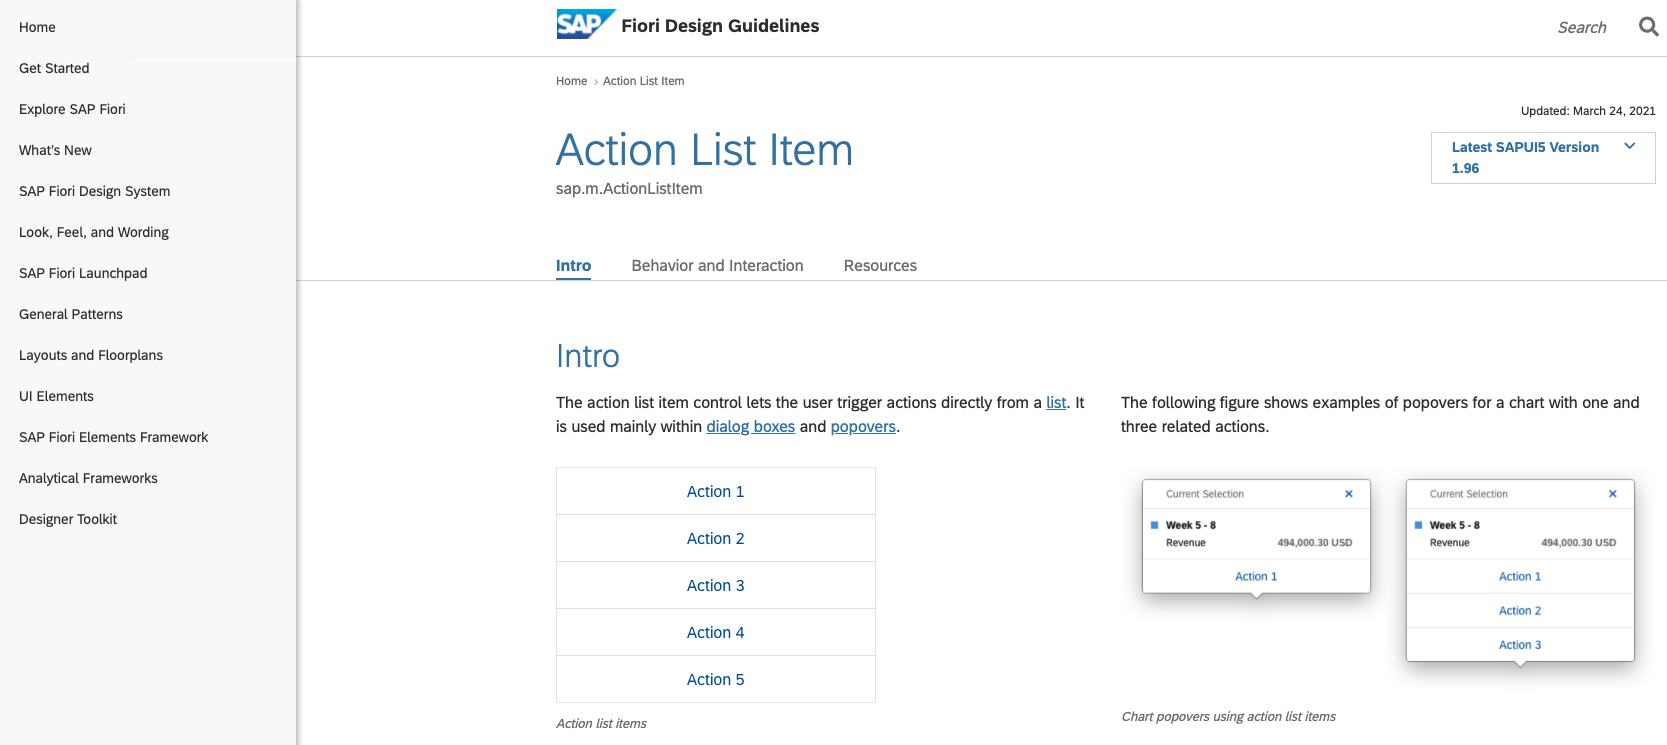
\includegraphics[width=\linewidth]{images/fiori_action-list_formal.png}}
\caption{SAP Fiori Action List formal guideline \cite{sap_fiori_nodate}}
\label{fiori_action_list}
\end{figure}
\newpage

\subsubsection{Usage guidelines} Usage guidelines help to understand how to use components. In addition, these guidelines explain how the corresponding parameters of a component work. This way, the user knows everything he needs to use the component in the product. \cite{vesselov_building_2019} \\
As can be seen in Figure \ref{atlassian_button}, the guideline provides guidance on where the component should be used. Sometimes usage guidelines also offer anti-patterns to the users. Anti-patterns tell users of the design system where they should not use that component.
\begin{figure}[htb]
\centerline{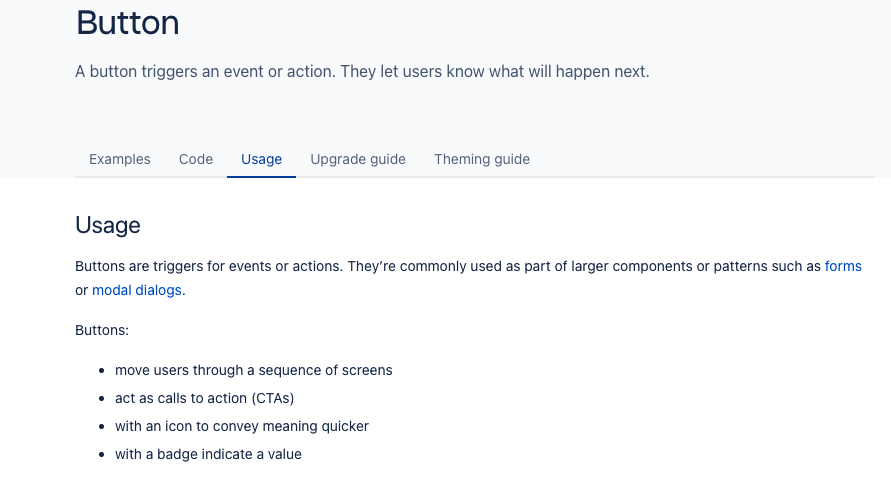
\includegraphics[width=\linewidth]{images/atlassian_button_usage.png}}
\caption{Atlassian Design System Button usage guideline \cite{atlassian_design_system_atlassian_nodate}}
\label{atlassian_button}
\end{figure}

\subsubsection{Technical guidelines} \label{tech_guideline}
\begin{wrapfigure}{r}{7cm}
	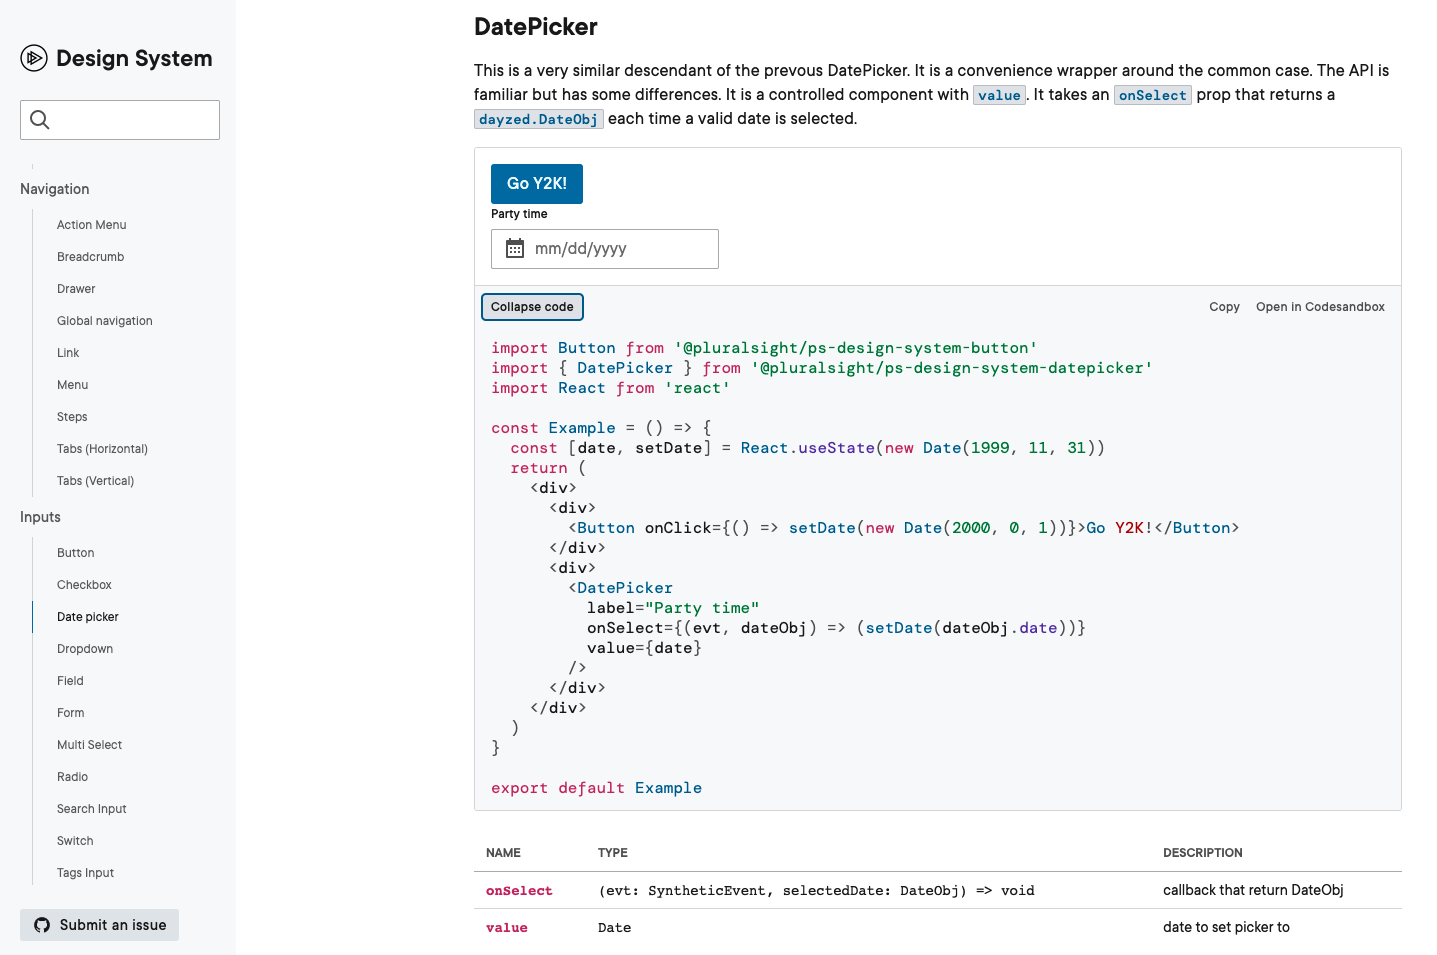
\includegraphics[width=7cm]{images/pluralsight_date-picker_technical.png}
	\caption{Pluralsight Design System Date picker technical guidelines \cite{pluralsight_ds_nodate}}
	\label{pluralsight_date_picker}
	\end{wrapfigure}
% Left here
This part of the guide is mainly intended for developers who are to implement the documented component in the software. Technical guidelines clarify ambiguities in implementation.  \cite{macdonald_practical_2019} \\
The same way as the corresponding parameters configure the appearance or behavior of a component. An often-found feature here is copying code snippets. This allows developers to immediately copy and paste the component code into their code. \cite{vesselov_building_2019} \\
Figure \ref{pluralsight_date_picker} shows a good example.The implementation of Pluralsight's Date Picker is explained very well here with a code example. The code snippets can be copied directly, opened, and tried out in a code sandbox.

\subsubsection{Related components} Linking components and patterns help the user explore the design system. Also, this can support the creative process for designers and developers. \\
Figure \ref{servicenow_accordion} is an example of a linked component in a design system. Such a representation of a linked component not only helps with creativity, but also lets developers and designers move more quickly through the collection of components. \\
This way, if there are problems with the implementation, the developer can quickly understand the relationship between the used components and resolve the issue. \cite{vesselov_building_2019}
\begin{figure}[htbp]
\centerline{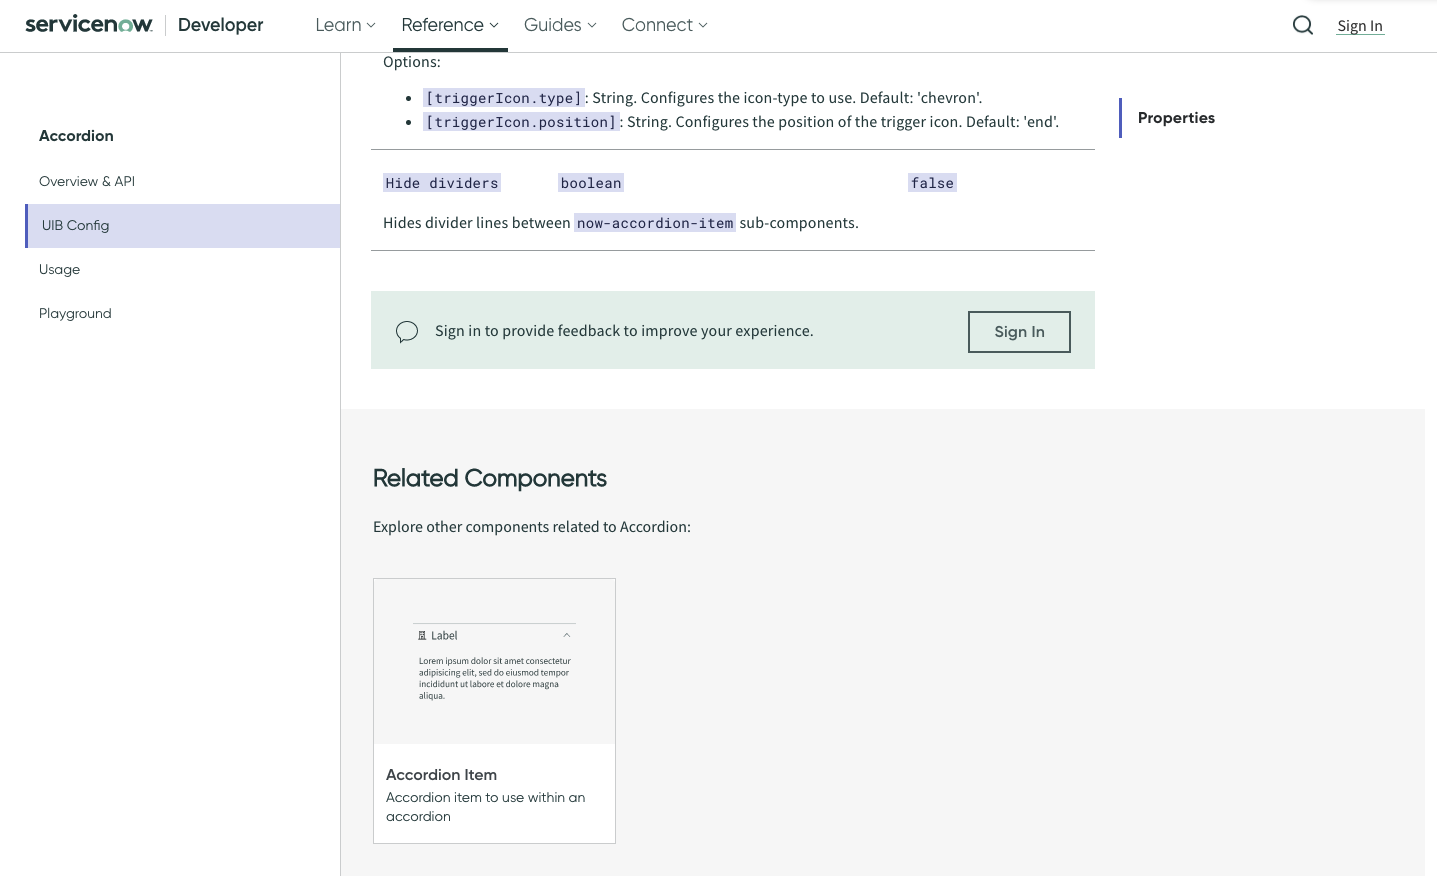
\includegraphics[height=150px]{images/servicenow_accordion_related.png}}
\caption{Servicenow Accordion related components \cite{servicenow_servicenow_nodate}}
\label{servicenow_accordion}
\end{figure}

\subsection{Design Principles}\label{design_principles}
Design principles should be a central consideration when building a design system. At the same time, the design principles should reflect the norms and values of the product organization. In doing so, the points established do not follow any rules, except that they are set collectively by the team. \\
Thus, these design principles serve as a basis for design discussion and decision-making. By simply self-explanatory principles, the designers and developers can quickly create new designs without a significant coordination effort. Often questions are taken as principles. This gives developers and designers the impulse to ask themselves whether they follow the design principles during the creation process. \cite{brignell_design_2022} \\
As an example, \citet{berners-lee_principles_2013} has developed design principles for the web: 
\begin{itemize}
\item \textbf{Simplicity} - Simple solutions are better solutions
\item \textbf{Modular Design} - Change things and it will only affect one part
\item \textbf{Being part of a Modular Design} - Realize you own the Design System
\item \textbf{Tolerance} - "Be liberal in what you require but conservative in what you do"
\item \textbf{Decentralization} - Don't produce bottlenecks, allow scaling in any direction
\item \textbf{Test of Independent Invention} - "Designing a system not to be modular in itself, but to be a part of an as-yet unspecified larger system."
\item \textbf{Principle of Least Power} - Use matching tools for the matching tasks
\end{itemize}
Design principles can be quite different. In this case, they are relatively technical, as the team wants to focus on this topic. Other organizations, such as Adobe with Adobe Spectrum, have people at the forefront. \cite{spectrum_adobe_spectrum_nodate} \\
Many underestimate the importance of these anchor points. Design principles play a central role in a design system.  The product team should not only build software based on these principles, but also gain an understanding of the big picture of the product organization. Therefore, the companies' design strategy is in line with their design principles. In this way, not only is the existing product organization aligned with the design principles, but new employees can also use them to integrate themselves more quickly into the product organization. Design principles are effective when they serve as a guide for the creative process.\cite{vesselov_building_2019} \\
First and foremost, a team must create design principles. A single person should not establish design principles on his or her own, even if it is possible to do so. Developing design principles as a large group reflects the creative thinking of everyone and helps align the entire company with these values. \\
Here, \citet{vesselov_building_2019} lay out a 5-step plan to iteratively create and continuously improve them. Figure 5 summarizes these  \ref{design_principles_steps} steps:
\newpage


\begin{figure}[htbp]
\centerline{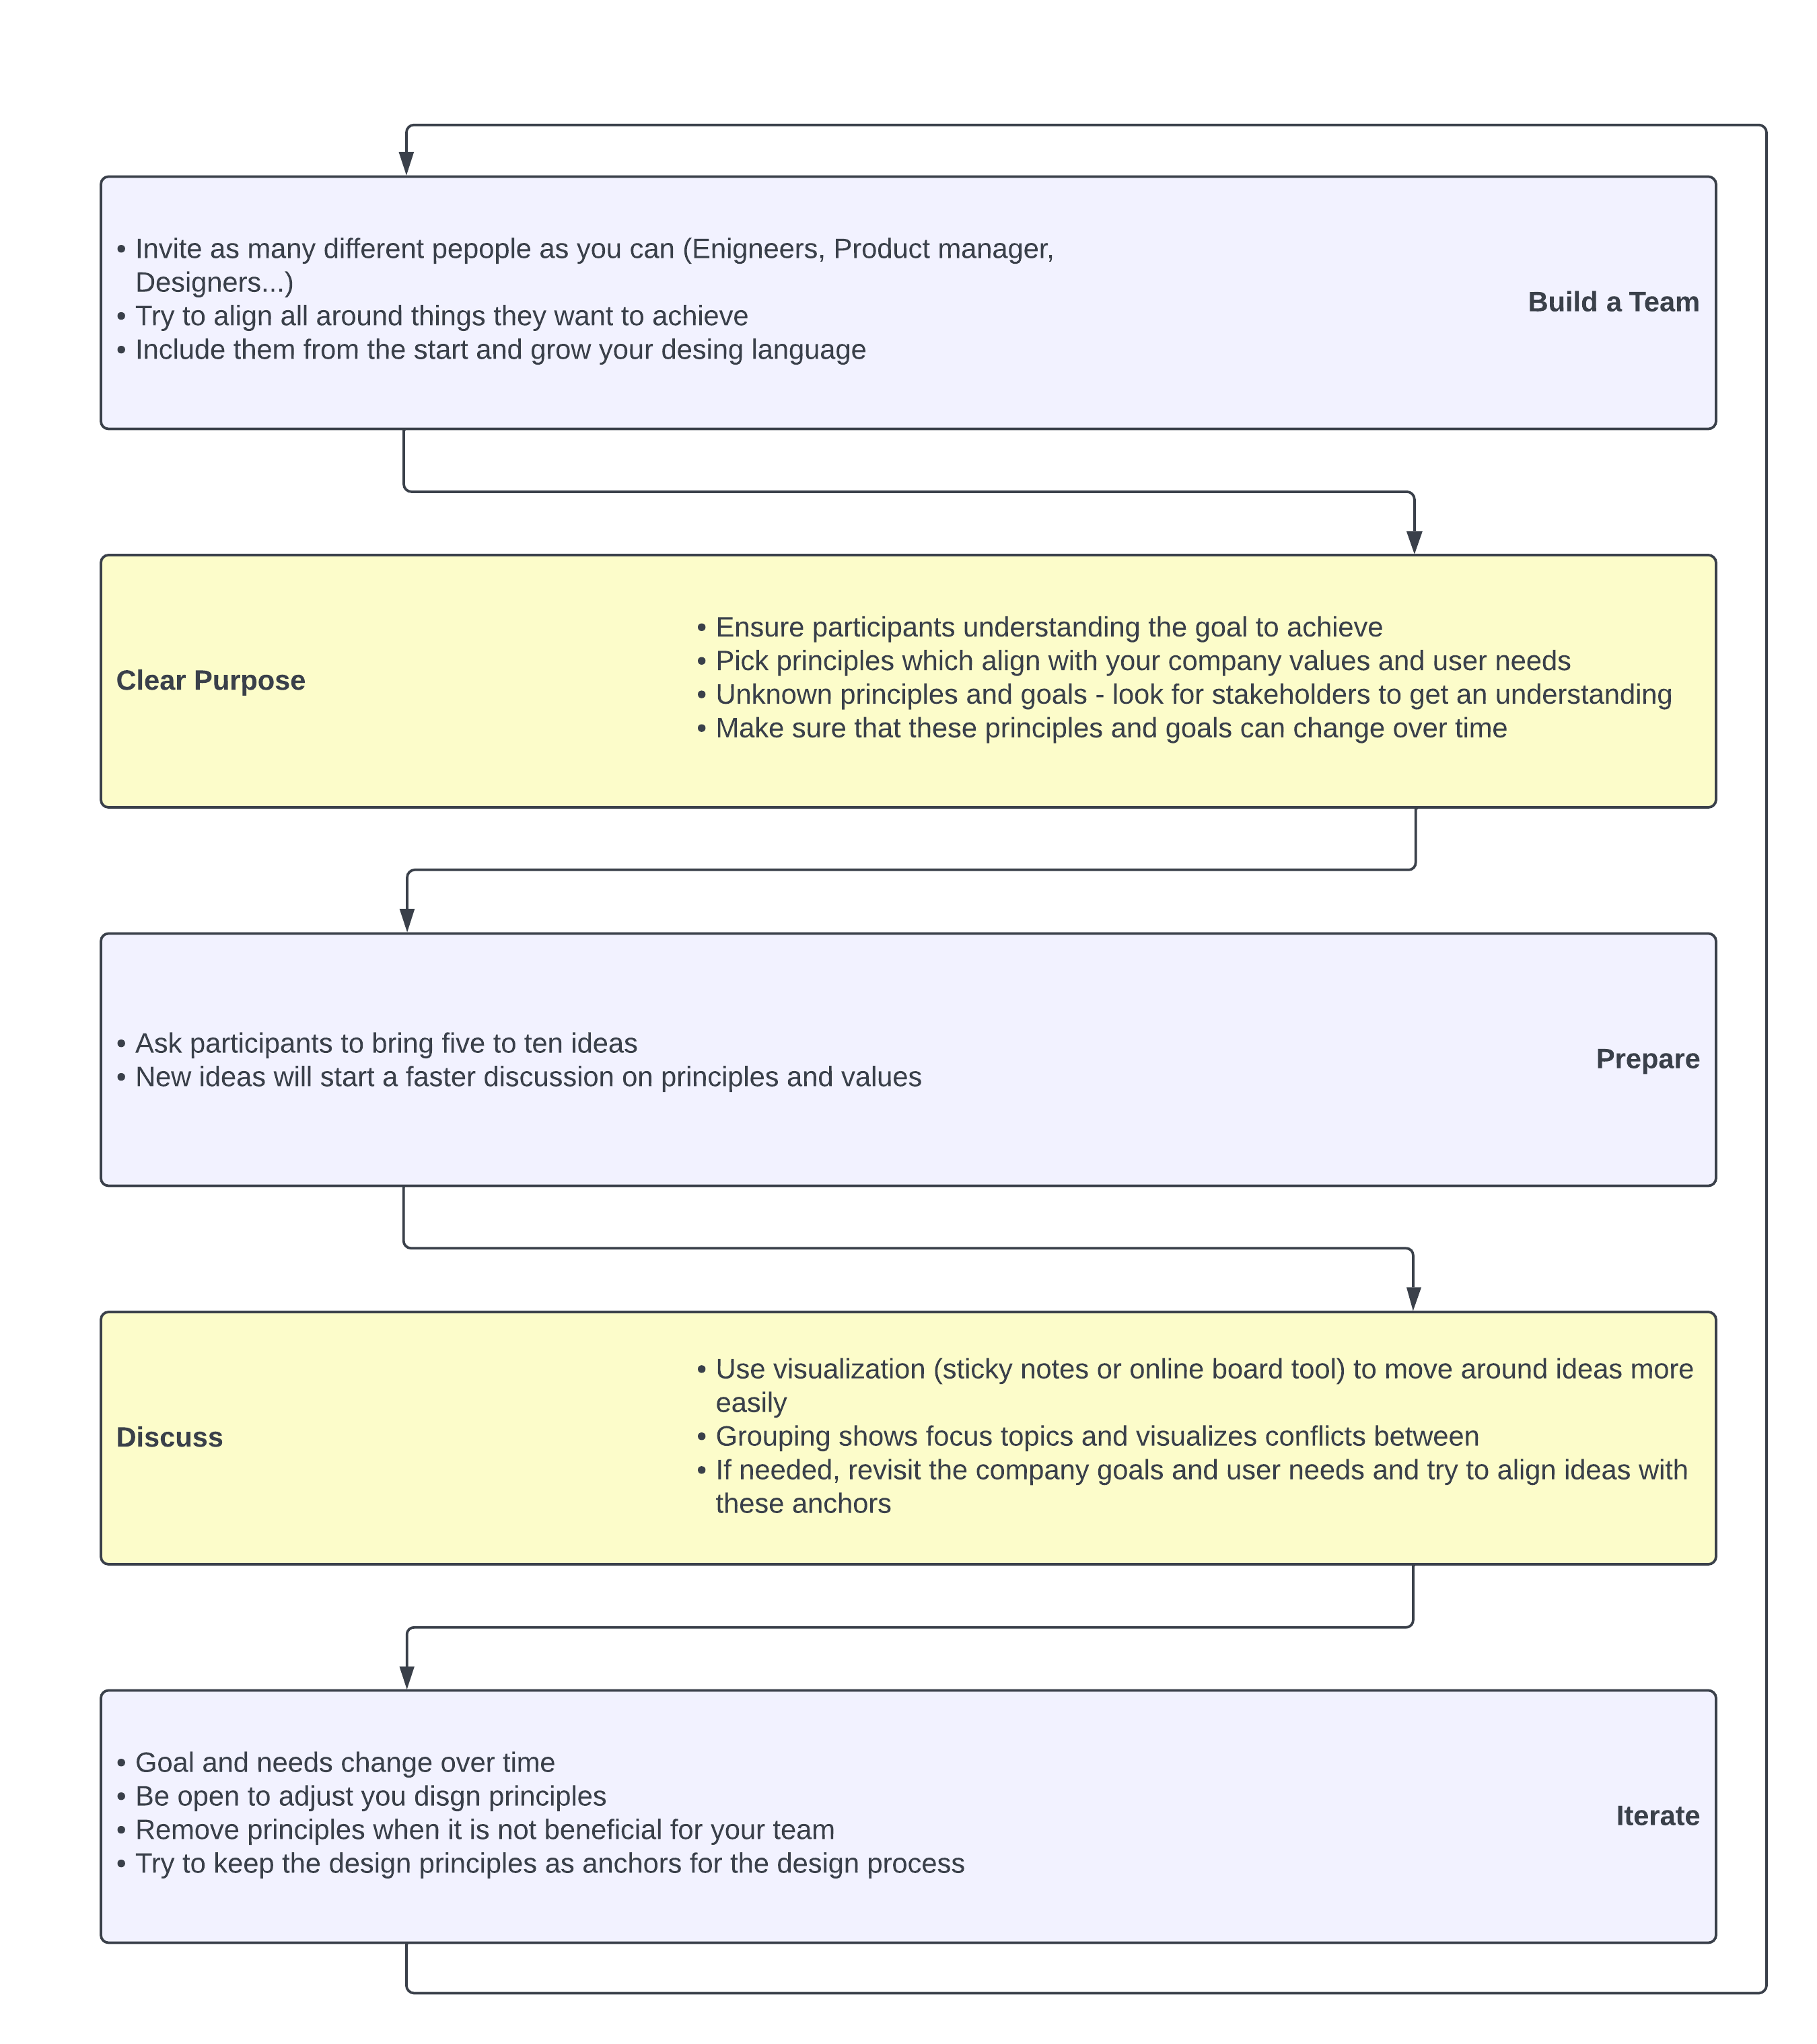
\includegraphics[width=\linewidth]{images/design_principles_steps.png}}
\caption{5 steps to introduce design principles inspired by  \citet{vesselov_building_2019}}
\label{design_principles_steps}
\end{figure}
Following these steps, a team creates design principles and implements an iterative process to update the design principles on a regular basis. \\
Next, the responsible team shares the values of the created design principles with the rest of the product organization. In this step, many design systems create so-called design blogs or design news. \\
They not only help the organization keep track of the design principles in their daily work. They also provide a platform to share updates with users. Moreover, there is an exchange on related topics on these platforms. This opens communication, in turn, helps to improve and keep the design system and principles up to date.  \cite{google_material_2022} \\
This chapter lays the foundation with the guidelines and design principles, while the next chapter will introduce another building block: the component library.
\subsection{Component Library}
The technical counterpart to the description guidelines and design principles is the component library. Both cannot exist in a design system without each other.  By definition, a component is "a constituent part"  of in this case a user interface. \cite{component_definition} Combined with library, which means a "collection of something", it results in a collection of important constituent parts for user interfaces. \cite{library_definition} \\
The definitions existing from the literature are as follows:
\begin{tcolorbox}[title=Definition of component library by \citet*{vesselov_building_2019}]
A set of styles and components that can be used and shared among a team. A component library consists of common core elements that are used throughout an application. [...] Component libraries may or may not include living code. [...] Unlike UI frameworks such as Bootstrap, component libraries are tailored to specific purposes, like an internal brand.
\end{tcolorbox}
In addition to components, there are also styling rules that also include layout specifications in component libraries. 
\begin{tcolorbox}[title=Definition of component library by \citet*{macdonald_practical_2019}]
Component libraries, UI libraries, or code libraries provide frontend code for UI components (a.k.a. widgets, modules, chunks, blocks). Internally, you might use a component library as a shared collection of UI snippets implementing patterns that anyone in the organization can contribute to building.
\end{tcolorbox}
An important point that emerges from these definitions is that component libraries have a clear focus on internal use. This is also the main difference to UI frameworks. \\
After reviewing various design systems, component libraries are divided into 4 categories:
\begin{itemize}
	\item \textbf{Layout} - Spacing and presentation of content placement on a site
	\item \textbf{Styles} - Color definitions, Typography, Icons
	\item \textbf{Components} - Reusable parts fulfilling one purpose
	\item \textbf{Patterns} - Combination of multiple components 
\end{itemize}

\subsubsection{Layout} \label{layout}
The foundation of any design system is the ability to place, move, or arrange elements on web pages. To achieve a consistent appearance in applications, it is important to align spacing and positioning in a central place. \\ 
For this purpose, so-called design tokens in form of CSS variables are often used. Similar to Tailwind (\url{https://tailwindcss.com/}), CSS classes implement design tokens and abstract them, so the developer does not need to use the variables natively. Thus, the developer does not need to know anything about CSS.  \\
Salesforce Lightning Design System, for example, lists all layout tools under \textbf{Utilities}. It sets sizes for text, simple boxes, and spacing between components. In fact, a sophisticated grid layout system can be seen as well. \\
\begin{figure}[hbtp]
	\centerline{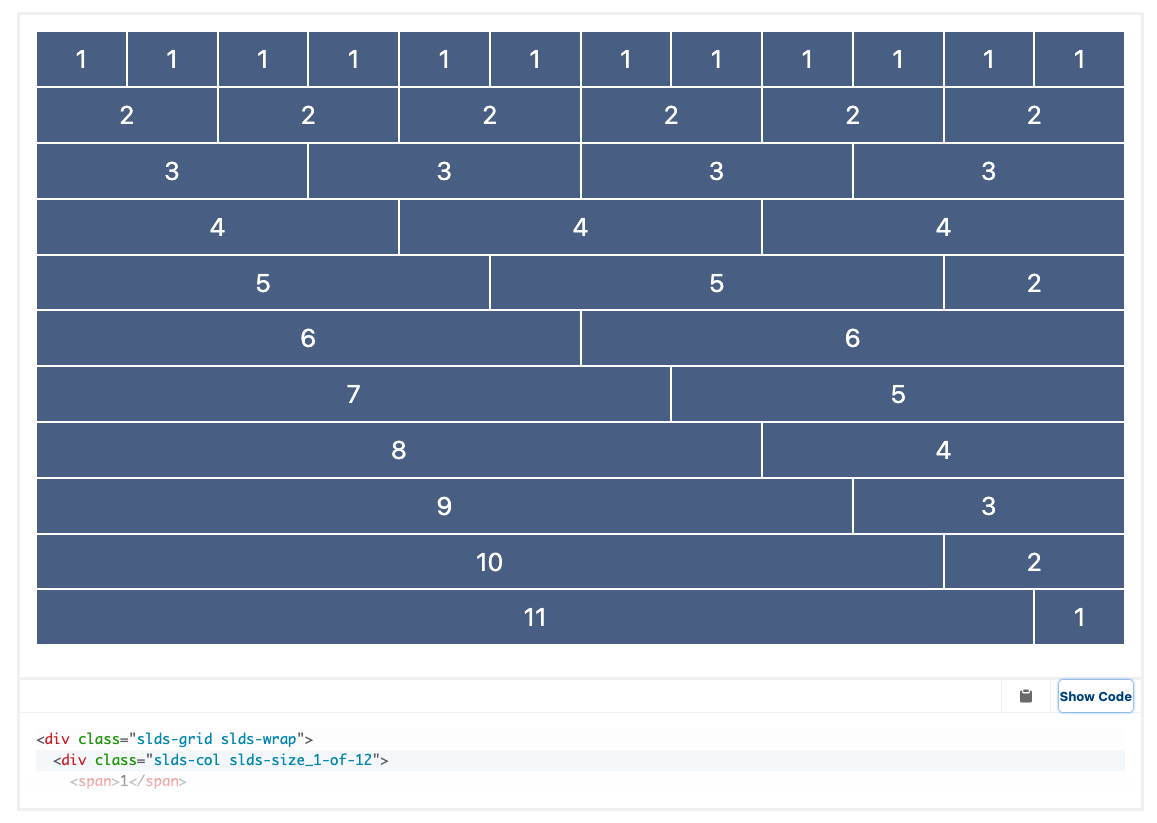
\includegraphics[width=\linewidth]{images/salesforce_lightning_layout.png}}
	\caption{Salesforce Lightning Design System grid layout \cite{lightning_design_system_lightning_nodate}}
	\label{salesforce_lightning_layout}
\end{figure} 

Figure \ref{salesforce_lightning_layout} shows that CSS classes achieve the desired layout. Furthermore, both dynamic and static layouts are supported. So the user has all possibilities to use the layout of the design system.\\
Besides the usual regulations for spacing and positioning, other points like visibility, scrollability or printability can also be described in the layout. Basically, all requirements for visible elements in the target system can be specified by the default layouting in the design system.

\subsubsection{Styles}
Styles are about colors, typography and icons. These topics may seem trivial, but it is important to make a connection to the chosen design principles. This helps to convey that design language in the other disciplines of the component library. \\
A style system provides enough freedom for design decisions so that the implemented products still have the possibility to have a unique look and feel. Some component libraries ensure this by allowing customization of basic style parameters.\cite{vesselov_building_2019}

\paragraph{Color}
A good first step is the introduction of a color system to build a design system. Colors are important for the aesthetics of a product.
Without changing the functionality or layout, the product team can change the colors until they fit the product. \\
\begin{figure}[htbp]
	\centerline{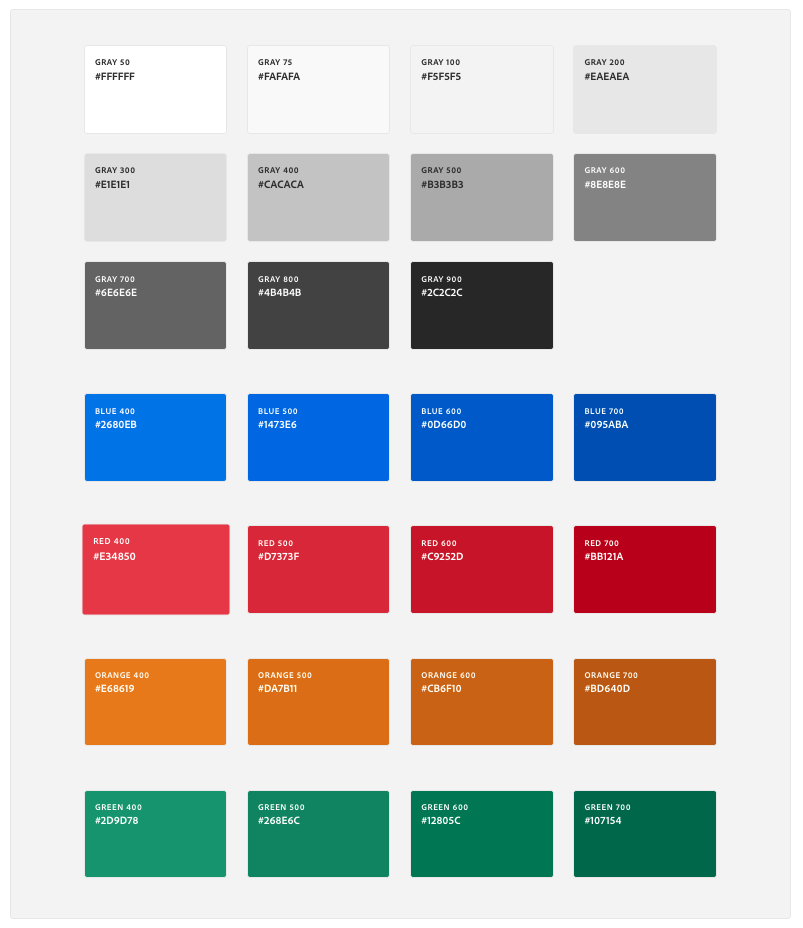
\includegraphics[height=8cm]{images/adobe_spectrum_color_palette.png}}
	\caption{Adobe Spectrum color palette \cite{spectrum_adobe_spectrum_nodate}}
	\label{adobe_spectrum_colors}
\end{figure}
It is always important to keep accessibility in mind when choosing colors. For a specific text size, it is important to maintain a certain contrast on colors. The WCAG (\url{https://www.w3.org/WAI/standards-guidelines/wcag/}) describes this contrast with two levels AA and AAA. This contrast is especially important if a product has several long paragraphs.  \\
Adobe's Spectrum Design System in Figure \ref{adobe_spectrum_colors} illustrates that design systems provide not just one color, but an entire color palette. The colors are often divided into primary, secondary, text color, background color, accent colors, shadows and so on. \\
Again, CSS variables with the appropriate names consume color tokens to provide them later for product implementation. The challenge is to offer a well-defined color palette, but at the same time not to overload the user. Too many colors quickly confuse users about which color to use for the feature. \cite{vesselov_building_2019}

\paragraph{Typography}
A typography system has two different categories. \\
First, there is typography for smaller text elements. Such elements consist of a maximum of three words. Examples are headings, buttons or labels. \\
Second, typography determines the appearance of long paragraphs. Paragraphs can have a different weight, size, or even a different font family altogether.
\begin{figure}[hbtp]
	\centerline{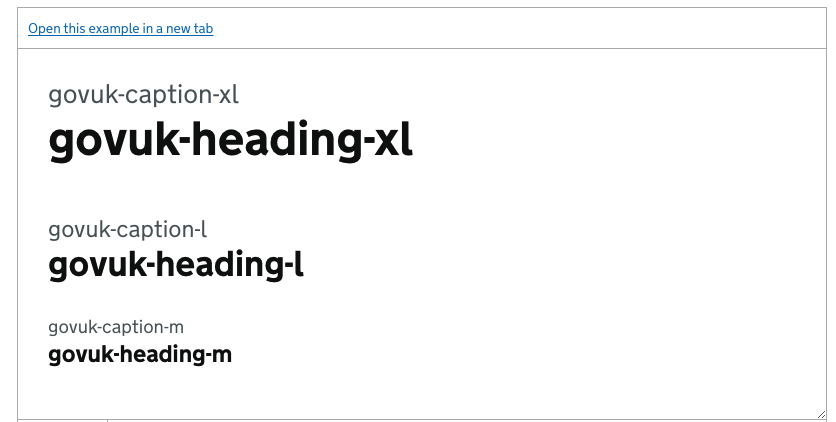
\includegraphics[height=5cm]{images/gov_uk_typo.png}}
	\caption{GOV.UK Design System caption typography example \cite{govuk_govuk_nodate}}
	\label{gov_uk_typo}
\end{figure} \\
In both cases, however, the general typography must follow the defined layout system. Texts rely on defined design features for spacing and padding. Figure \ref{gov_uk_typo} shows a helpful tool, an overview of all typography options supports the selection of the right design.  \cite{vesselov_building_2019}


\paragraph{Iconography}
The Icongraphy is a bit of a specialty in a design system. It may not seem to be important for a product but icons often deliver a lot of the overall design language to the end user. \\
Although icons are important to design language, it is not always necessary to create new iconography. A good start is to use an iconography that is already widely used. Later, a custom iconography offers a lot of potential to visualize the company's design language in it. \\
As with other parts of a design system, documentation is key. Focus on how to create new icons, what proportions and shapes. If done right, it's an easy step to introduce new icons into the iconography. 
\\
To make them accessible to the team, an iconography describes how to add them to the product. As in the technical guidelines in \ref{tech_guideline}, a code snippet explains their use to the developer. \cite{vesselov_building_2019}

\subsubsection{Components}
Components are the heart of a component library. Moreover the building blocks for applications. They are built with all the tools and fundamentals just presented.Components are highly reusable and as flexible.  \\
\begin{figure}[hbtp]
	\centerline{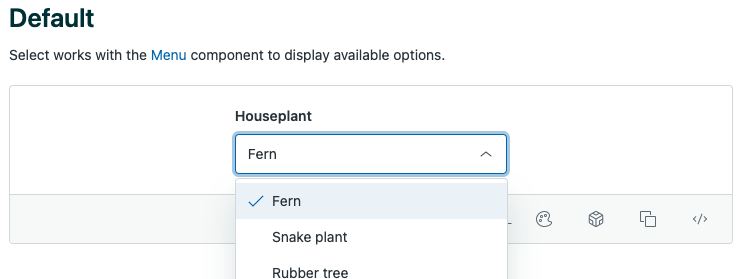
\includegraphics[height=5cm]{images/zendesk_component_example.png}}
	\caption{Zendesk Garden dropdown component \cite{zendesk_garden_zendesk_nodate}}
	\label{zen_garden_component}
\end{figure}

Combinations of layout and style specifications result in components for different use cases. Also, Figure \ref{zen_garden_component} shows that a component that is widely used in different design systems is a dropdown component. Because native dropdowns are often unable to meet full user experience requirements, component libraries have often replicated this component.\\
By using these predefined components in applications, the developer ensures that the guidelines are adhered to. For certain combinations of components in an application, there is another term called patterns, which is explained in more detail in chapter \ref{patterns}. \\

\begin{figure}[hbtp]
	\centerline{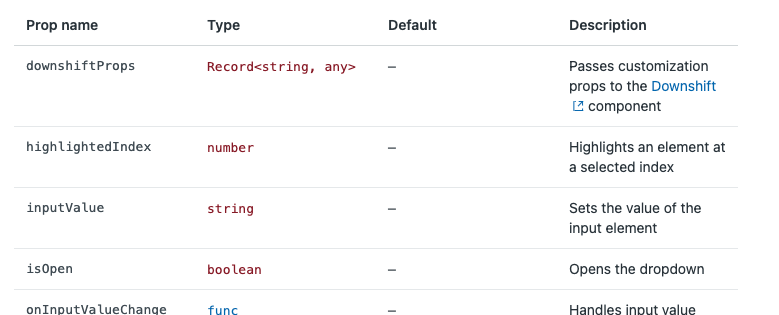
\includegraphics[height=5cm]{images/zendesk_component_interface.png}}
	\caption{Zendesk Garden dropdown interface \cite{zendesk_garden_zendesk_nodate}}
	\label{zen_garden_interface}
\end{figure}
To achieve flexibility and reusability, it is important to always have the component's interfaces in mind. Well-defined interfaces are the key to successful components. A possible solution, as in Figure \ref{zen_garden_interface}, is good interface documentation. A simple table with property values, the expected type and a short description is sufficient. In some design systems, the developer can change these input properties in a live demo so that the developer can see the changes immediately.\\
As with other parts of a design system, documentation is key. To get well-documented interfaces, always involve the engineers who are actually building the product to receive their feedback.  A well-structured and systematic approach to how a component works helps developers use the components.  \cite{vesselov_building_2019}\\
The above-mentioned components alone are not enough. Sometimes it takes more than one component to get the job done. The next chapter explains how patterns achieve documentation of a complex component construct. 

\subsubsection{Patterns} \label{patterns}
Often, a combination of certain components is used over and over again in different places and even in different applications. To cover this use case, a design system has a concept called patterns.\\ 
Patterns specify a combination of several components and document the composition of these components. Patterns are an extended documentation to reproduce a certain combination of components in an application. \\
\begin{figure}[htbp]
	\centerline{
\includegraphics[height=7.5cm]{images/atlassian_abstract_form.png}}
	\caption{Atalssian Design System abstract form layout \cite{atlassian_design_system_atlassian_nodate}}
	\label{atlassian_form_layout}
\end{figure}
Atlassian's design system provides an excellent example of a pattern with its forms. Figure \ref{atlassian_form_layout} shows an abstract visualisation of how input fields and buttons should be placed when a form is on a single page. This abstraction leaves no room for interpretation, and developers and designers can continue with their work. \\
Patterns refer not only to the interaction of components, but also to the switching of visualization due to changes in a user's permissions, for example. A pattern documents all UI changes related to the user experience, no matter how small. \cite{vesselov_building_2019} \\
Most often, patterns appear in the general navigation of applications. Such navigation patterns evolve naturally from introducing them into products and grow iteratively with more and more feedback from the product development team.\\
A good example for a pattern is the navigation bar. By combining components such as buttons, dropdowns, and images, a navigation bar is created. Together with skeleton code around these components documented in a pattern, they form a complete navigation area within an application. 
